We verify a standard C implementation of Dijkstra's algorithm.
We first sketch our proof in some detail with an emphasis on our loop invariants,
then uncover and remedy a subtle overflow bug, and finish with a discussion
of related work.

\subsection{Verified Dijkstra's algorithm in C}
\label{sec:dijkoverview}

Figure~\ref{fig:decorated} shows the code and proof
sketch of Dijkstra's algorithm.
{\color{red}Red} text in an annotation indicates changes compared to the
annotation immediately prior.
Our code is implemented exactly
as suggested by CLRS~\cite{clrs}, so we refer readers there for a
general discussion of the algorithm.
The adjacency-matrix-represented graph~$\gamma$ of \texttt{size} vertices
is passed as the parameter \texttt{g} along with the source vertex \texttt{src}
and two allocated arrays \texttt{dist} and \texttt{prev}.
The spatial predicate $\mathsf{array}(\texttt{x},\vec{v})$, which connects
an array pointer \texttt{x} with its contents $\vec{v}$, is standard and unexciting.
$\mathsf{PQ}(\texttt{pq},\m{heap})$ is the spatial
representation of our priority queue (PQ) and
$\mathsf{Item}(\texttt{i},\m{(key, pri, data)})$
lays out a struct that we use to interact with the PQ;
we leave the management of the PQ to the operations described in~\S\ref{sec:binheap}.
Of greater interest is $\mathsf{AdjMat}(\texttt{g},\gamma)$, which as explained in~\S\ref{sec:newspatial}, links 
the concrete memory values of~\texttt{g} to an abstract mathematical
graph~$\gamma$, which in turn exposes an interface in the
language of graph theory (\emph{e.g.}, vertices, edges, labels).  Graph~$\gamma$ contains 
the general adjacency matrix restrictions given in \S\ref{sec:adjmatpure} along with some further
Dijkstra-specific restrictions to be explained in \S\ref{sec:dijkoverflow}.
We verify Dijkstra
three times using different adjacency-matrix representations as explained in \S\ref{sec:newspatial}.
Thanks to some careful engineering, the C code and
the Coq verification are both almost completely agnostic to
the form of representation. The only variation between implementations
is when reading a cell (line~\ref{code:cost}), so we
refactor this out into a straightforward helper method and
verify it separately; accordingly, the proof bases for the three variants differ by less than 1\%.
%\note{We also demonstrated that our pure reasoning was isolated from our spatial reasoning by verifying three versions of~C~code with slightly different memory layouts for adjacency matrices with the same pure theorems (our proof base for these versions differs by , exactly for the portion of the~C~code that accesses the graph representation in memory)}


\begin{figure}[t]

\begin{lstlisting}[mathescape=true,showlines=true]
void dijkstra (int **g, int src, int *dist,
               int *prev, int size, int inf {
$\color{OliveGreen}//~\braces{\p{AdjMat}(\texttt{g},\gamma) *
\mathsf{array}(\texttt{dist}, \_) * \mathsf{array}(\texttt{prev}, \_)}$
 Item* temp = (Item*) mallocN(sizeof(Item));
 int* keys = mallocN (size * sizeof (int));
 PQ* pq = pq_make(size); int i, j, u, cost;
 for (i = 0; i < size; i++)
 { dist[i] = inf; prev[i] = inf; keys[i] = pq_push(pq,inf,i); } $\label{code:assigninf}$
 dist[src]= 0; prev[src]= src; pq_edit_priority(pq,keys[src],0);
 while (pq_size(pq) > 0) {
$\color{OliveGreen}//~\braces{{\color{red}\exists \m{dist}, \m{prev}, \m{popped}, \m{heap}}.~\p{AdjMat}(\texttt{g},\gamma) * {\color{red}\p{PQ}(\texttt{pq},\m{heap})} *
{\color{red}\mathsf{Item}(\texttt{temp}, \_)} * \null \\
\mathsf{array}(\texttt{dist},{\color{red}\m{dist}}) *
\mathsf{array}(\texttt{prev}, {\color{red}\m{prev}}) *
{\color{red}\mathsf{array}(\texttt{keys}, \m{keys}}) /| \null \\
{\color{red}\m{linked\_correctly}(\gamma, \m{heap}, \m{keys}, \m{dist}, \m{popped})} /| \null \\
{\color{red}\m{dijk\_correct}(\gamma,\texttt{src},\m{popped},\m{prev},\m{dist})}}$ $\label{code:whileinv}$
  pq_pop(pq, temp); u = temp->data; $\label{code:pop}$
  for (i = 0; i < size; i++) {
$\color{OliveGreen}//~\braces{{\color{red}\exists \m{dist'}, \m{prev'}, \m{heap'}}.~\p{AdjMat}(\texttt{g},\gamma) * \p{PQ}(\texttt{pq},{\color{red}\m{heap'}}) * \null \\
\mathsf{array}(\texttt{dist},\m{\color{red}dist'}) *
\mathsf{array}(\texttt{prev}, \m{\color{red}prev'}) *
\mathsf{array}(\texttt{keys}, \m{keys}) * \null \\
\mathsf{Item}(\texttt{temp}, \m{\color{red}(\texttt{keys[u]}, \texttt{dist[u]}, \texttt{u})}) /|
\m{\color{red}min(\texttt{dist[u]}, \m{heap'})} /| \null \\
{\m{linked\_correctly}(\gamma, \m{\color{red}heap'}, \m{keys}, \m{\color{red}dist'},
{\color{red}\m{popped} \uplus \{\texttt{u}\}})} /| \null \\
{\color{red}\m{dijk\_correct\_weak}({\color{OliveGreen}\gamma, \texttt{src}}, \m{popped} \uplus \{\texttt{u}\}, \m{prev'}, \m{dist'}, \texttt{i}, \texttt{u})}}$ $\label{code:forinv}$
   cost = getCell(g, u, i); $\label{code:cost}$
   if (cost < inf) {
    if (dist[i] > dist[u] + cost) { $\label{code:overflow}$
     dist[i] = dist[u] + cost; prev[i] = u; $\label{code:update1}$
     pq_edit_priority(pq, keys[i], dist[i]); $\label{code:update2}$
  }}}} $\color{OliveGreen}//~\braces{{\color{red}\exists \m{dist''}, \m{prev''}}.~\p{AdjMat}(\texttt{g},\gamma) * \p{PQ}(\texttt{pq},\m{\color{red}\emptyset}) * {\mathsf{Item}(\texttt{temp}, {\color{red}\_})} * \null \\
 \mathsf{array}(\texttt{dist},\m{\color{red}dist''}) *
 \mathsf{array}(\texttt{prev}, \m{\color{red}prev''}) *
 \mathsf{array}(\texttt{keys}, \m{keys}) /| \null \\
{\color{red}\forall \m{dst}.~0 \le \m{dst} < \texttt{size} -> \m{inv\_popped}}(\gamma, \m{src}, {\color{red}\m{\gamma.V}, \m{prev''}, \m{dist''}, \m{dst}})}$ $\label{code:end}$
 freeN (temp); pq_free (pq); freeN (keys); return; }
\end{lstlisting}
\vspace{-1em}
\caption{C code and proof sketch for Dijkstra's Algorithm.}
\vspace{-1em}
\label{fig:decorated}
\end{figure}



\hide{
$\color{OliveGreen}//~\braces{{\color{red}\exists \m{dist''}, \m{prev''},\m{heap''}}.~\p{AdjMat}(\texttt{g},\gamma) * \p{PQ}(\texttt{pq},\m{\color{red}heap''}) *
  \mathsf{array}(\texttt{dist},\m{\color{red}dist''}) * \null \\
  \mathsf{array}(\texttt{prev}, \m{\color{red}prev''}) *
  \mathsf{array}(\texttt{keys}, \m{keys}) *
  \mathsf{Item}(\texttt{temp}, \m{(\texttt{keys[u]}, \texttt{dist[u]}, \texttt{u})} /| \null \\
  \m{min(\texttt{dist[u]}, \m{heap'})} /|
  {\color{red}\m{heap''} = \m{heap'} [\texttt{keys[i]} \mapsto (\texttt{dist[i]},\texttt{i})]} /| \null \\
  {\m{\color{red}dijk\_correct}(\gamma, \texttt{src}, \m{popped'}, \m{\color{red}prev''}, \m{\color{red}dist''})}}$ $\label{code:caughtup}$
}


\hide{In general, these spatial representations are simple enough
that they pose no special
challenge in the proof. Therefore, in our discussion below, we
will not focus on issues such as making sure an array dereference is in bounds.
} %hide

Dijkstra's algorithm uses a PQ to greedily choose the
cheapest unoptimized vertex on line~\ref{code:pop}. The
best-known distances to vertices are expected to improve as
various edges are relaxed, and such improvements need to be logged in the PQ:
Dijkstra's algorithm implicitly assumes that its~PQ supports the additional
operation \texttt{decrease\_priority}.
Our ``advanced''~PQ~(\S\ref{sec:modpri})
supports this operation in logarithmic time with the
\texttt{pq\_edit\_priority} function\footnote{Because
\texttt{decrease\_priority} is relatively complex to implement,
several popular
workarounds (\emph{e.g.}~\cite{arthur}) use simpler PQs at the cost
of decreased performance.}.
% each \texttt{pop\_min} now takes $\bigO(n)$ time.

%Note that \texttt{dist} already tracks the best-known cost
%to any vertex (line~\ref{code:update1}). Maintain a list of
%vertices that have been optimized.
%Find the cheapest unoptimized vertex by
%iterating over \texttt{dist} while rejecting optimized items.
%Neat, but far too slow.

The first nine lines are standard setup.
The \emph{keys} array, assigned on line~\ref{code:assigninf},
is thereafter a mathematical constant.
The pure predicate \m{linked\_correctly} contains the plumbing connecting the
various mathematical arrays.
The verification turns on the loop
invariants on lines~\ref{code:whileinv} and~\ref{code:forinv}.  The pure \texttt{while} invariant $\m{dijk\_correct}(\gamma, \m{src}, \m{popped}, \m{prev}, \m{dist})$ essentially unfolds into:
\[
\begin{array}{lcl}
\forall \m{dst}.~\m{dst} \in \gamma & -> & \m{inv\_popped}(\gamma, \m{src}, \m{popped}, \m{prev}, \m{dist}, \m{dst}) /| \null \\
&&\m{inv\_unpopped}(\gamma, \m{src}, \m{popped}, \m{prev}, \m{dist}, \m{dst}) /| \null \\
&&\m{inv\_unseen}(\gamma, \m{src}, \m{popped}, \m{prev}, \m{dist}, \m{dst})
\end{array}
\]
That is, a destination vertex $\m{dst}$ falls into one of three
categories:
\begin{enumerate}
\item $\m{inv\_popped}$: if $\m{dst} \in \m{popped}$, 
then $\m{dst}$ has been fully processed, \emph{i.e.} \m{dst} is reachable from~$\m{src}$
via a globally-optimal path $p$ whose vertices are all in $\m{popped}$.  Path $p$ has been logged in \m{prev} and $p$'s cost is given in \m{dist}.

%has a globally optimal path
%from
% whose edges are logged in  and whose cost is
%; all vertices in this path are also popped.
%is reachable, meaning that a globally optimal
%path ~to~$\m{dst}$ exists, the cost of this path is logged , all vertices visited by the path are also popped,
%and the links of the path are logged in.

\item $\m{inv\_unpopped}$: if $\m{dst} \not \in \m{popped}$, but its known $\m{dist}$ance is less than
\texttt{inf}, then $\m{dst}$ is reachable in one step from a popped vertex \m{mom}.
This route is locally optimal: we cannot improve the cost via an alternate popped vertex.
Moreover, \m{prev} logs
\m{mom} as the best-known way to reach $\m{dst}$, and \m{dist}
logs the path cost via \m{mom} as the best-known cost.
\item $\m{inv\_unseen}$: if $\m{dst} \not \in \m{popped}$ and its known $\m{dist}$ance is \texttt{inf}, then
there is no edge from any $\m{popped}$ vertex to $\m{dst}$; in other words, $\m{dst}$ is located deeper in the graph
than has yet been explored.
\end{enumerate}
After line~\ref{code:pop},
the above invariant is no longer true: a minimum-cost item~\m{u} has been
popped from the PQ, and so the \m{dist} and \m{prev} arrays need to be
updated to account for this pop. The \texttt{for} loop does exactly this repair work.
Its pure invariant
$\m{dijk\_correct\_weak}(\gamma, \m{src}, \m{popped}, \m{prev}, \m{dist}, \m{u}, \m{i})$ essentially unfolds into:
\[
\begin{array}{lcl}
\big(\forall \m{dst}.~\m{dst} \in \gamma & -> & \m{inv\_popped}(\gamma, \m{src}, \m{popped}, \m{prev}, \m{dist}, \m{dst})\big) /| \null \\
\big(\forall \m{dst}.~\texttt{0} \le \m{dst} < \m{i} & -> & \m{inv\_unpopped}(\gamma, \m{src}, \m{popped}, \m{prev}, \m{dist}, \m{dst}) /| \null \\
&& \m{inv\_unseen}(\gamma, \m{src}, \m{popped}, \m{prev}, \m{dist}, \m{dst}) \big) /| \null \\
\big(\forall \m{dst}.~\m{i} \le \m{dst} < \texttt{size} & -> & \m{inv\_unpopped\_weak}(\gamma, \m{src}, \m{popped}, \m{prev}, \m{dist}, \m{dst}, \m{u}) /| \null \\
&&\m{inv\_unseen\_weak}(\gamma, \m{src}, \m{popped}, \m{prev}, \m{dist}, \m{dst}, \m{u}) \big)
\end{array}
\]
We now have five cases, many of which are familiar from $\m{dijk\_correct}$:
\begin{enumerate}
\item $\m{inv\_popped}$: as before; if $\m{dst} \in \m{popped}$, then it has been fully processed.  
For all ``previously-popped vertices'' (\emph{i.e., }except for~\m{u}),
this is trivial from $\m{dijk\_correct}$. For~\m{u} itself, we reach the heart of Dijkstra's correctness:
the locally-optimal path to the cheapest unpopped vertex is
\emph{globally} optimal.
%the cost to the unpopped vertex with minimum cost cannot be further improved.  %The associated entailment is not trivial.
\item $\m{inv\_unpopped}$ (less than \m{i}): as before; if $\m{dst}$ is reachable in
one hop from a popped vertex \m{mom}, where now \m{mom} could be \m{u}. Initially this is trivial since $\m{i}=0$, and we restore it as \m{i} increments by updating costs when they can be improved, as on lines~\ref{code:update1}~and~\ref{code:update2}.
\item $\m{inv\_unseen}$ (less than \m{i}): as before; some previously unseen neighbors of \m{u} may be transferred to unpopped status.  This is also restored as \m{i} increments.
\item $\m{inv\_unpopped\_weak}$ (between \m{i} and \texttt{size}):
if $\m{dst}$ is reachable in one hop from a previously-popped vertex \m{mom},
with potentially further improvements possible via~\m{u}.
As~$\m{i}$ increments, we strengthen it
into $\m{inv\_unpopped}$ after considering whether routing via
\m{u} improves the best-known cost to~\m{dst}.
\item $\m{inv\_unseen\_weak}$ (between \m{i} and \texttt{size}):
no edge exists from any previously-popped vertex to
$\m{dst}$, but there may be one from~\m{u}.
As~$\m{i}$ increments, we consider whether routing via~\m{u}
reveals a path to~\m{dst}.
This is strengthened into
$\m{inv\_unpopped}$ if so, and into
$\m{inv\_unseen}$ if not.
\end{enumerate}
At the end of the \texttt{for} loop
the fourth and fifth cases fall away
(\texttt{\m{i}~=~size}), and the PQ and the \m{dist} and \m{prev} arrays
finish ``catching up'' to the pop on line~\ref{code:pop}.
This allows us to infer
the \texttt{while} invariant $\m{dijk\_correct}$,
and thus continue the \texttt{while} loop.
The \texttt{while} loop itself breaks when all vertices have been popped
and processed. The second and third clauses of the \texttt{while} loop invariant
$\m{dijk\_correct}$ then fall away, as seen on line \ref{code:end}:
all vertices satisfy \m{inv\_popped}, and are either optimally reachable or altogether unreachable.
We are done.

\hide{

While loop's invariant, which is stated on line
and explained further in Figure~\ref{fig:defns}.


This three-part invariant is trivially true before the while loop.
On line~\ref{code:pop}, the minimal vertex from the priority queue is popped,
thus breaking the invariant.

First, we must show that the minimal vertex $\m{u}$
obeys $\m{inv\_popped}$. \emph{i.e.}, show that the locally
optimal path to $\m{u}$ is, in fact, globally optimal.
This comes from blah blah blah

\newcommand{\s}{11}
\begin{figure}[htbp]
  \centering
  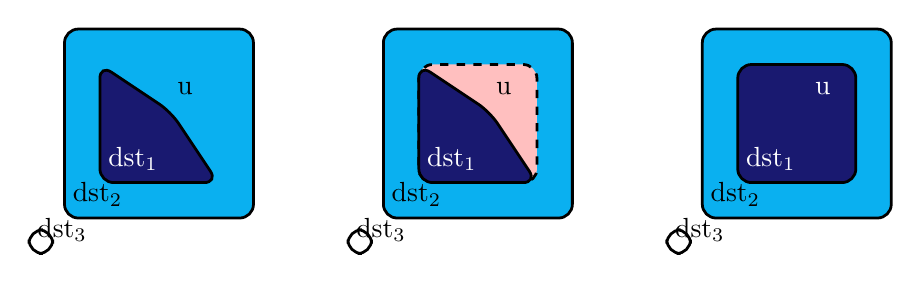
\begin{tikzpicture}[x=0.3cm, y=0.3cm,
      popped/.style={rounded corners=5pt, line width=1pt, draw, fill=MidnightBlue},
      fringe/.style={rounded corners=5pt, line width=1pt, draw, fill=ProcessBlue},
      popping/.style={rounded corners=5pt, line width=1pt, draw, dashed, fill=pink},
      unseen/.style={rounded corners=5pt, line width=1pt, draw}]
    \draw[unseen] (0,0) -- (\s,0) -- (\s,\s) -- (0,\s) -- cycle;
    \draw[fringe] (1.5,1.5) -- (9.5,1.5) -- (9.5,9.5) -- (1.5,9.5) -- cycle;
    \draw[popped] (3,3) -- (8,3) -- (6,6) -- (3,8) -- cycle;
    \node at (1.4,1) {dst$_3$};
    \node at (2.9,2.5) {dst$_2$};
    \node at (4.4,4) {\color{white}dst$_1$};
    \node at (6.6,7) {u};
    \tikzset{shift={(13.5,0)}}

    \draw[unseen] (0,0) -- (\s,0) -- (\s,\s) -- (0,\s) -- cycle;
    \draw[fringe] (1.5,1.5) -- (9.5,1.5) -- (9.5,9.5) -- (1.5,9.5) -- cycle;
    \draw[popping] (3,3) -- (8,3) -- (8,8) -- (3,8) -- cycle;
    \draw[popped] (3,3) -- (8,3) -- (6,6) -- (3,8) -- cycle;
    \node at (1.4,1) {dst$_3$};
    \node at (2.9,2.5) {dst$_2$};
    \node at (4.4,4) {\color{white}dst$_1$};
    \node at (6.6,7) {u};

    \tikzset{shift={(13.5,0)}}

    \draw[unseen] (0,0) -- (\s,0) -- (\s,\s) -- (0,\s) -- cycle;
    \draw[fringe] (1.5,1.5) -- (9.5,1.5) -- (9.5,9.5) -- (1.5,9.5) -- cycle;
    \draw[popped] (3,3) -- (8,3) -- (8,8) -- (3,8) -- cycle;
    \node at (1.4,1) {dst$_3$};
    \node at (2.9,2.5) {dst$_2$};
    \node at (4.4,4) {\color{white}dst$_1$};
    \node at (6.6,7) {\color{white}u};
  \end{tikzpicture}
  \caption{Popping $\m{u}$}
\end{figure}

Next, we must account for the ripple effect that popping
$\m{u}$ could have had on the other vertices.
In particular, it is possible that a vertex obeying $\m{inv\_unpopped}$ can
improve its cost via $\m{u}$, and that an unreachable vertex
obeying $\m{inv\_unseen}$ can now be reached via $\m{u}$.
The for loop repairs these breakages by
checking if a path via $\m{u}$ is an improvement for such vertices, and, if so,
edits both arrays and the priority queue as seen on line~\ref{code:update}.

The for loop's invariant is similar to that of the while loop---$\m{inv\_unseen}$
and $\m{inv\_popped}$ are preserved as-is, modulo the popping of
$\m{u}$ as discussed above. The key edit is in $\m{inv\_unpopped}$. blah blah blah

}

Dijkstra's algorithm clearly cannot work when a path
cost is greater than \texttt{INT\_MAX}.  A reasonable-looking restriction 
is to bound edge costs by 
$\left\lfloor\frac{\texttt{INT\_MAX}}{\texttt{size}-1}\right\rfloor$, since 
the longest optimal path has $\texttt{size}-1$ links and so the 
most expensive possible path costs no more than \texttt{INT\_MAX}.  
However, this has two flaws.  First, since we are writing real code in~C, 
rather than pseudocode in an idealized setting, we must reserve some 
concrete \texttt{int} value \texttt{inf} for ``infinity'', which has 
the special semantics that, if the best-known distance to a vertex~\m{x}
is \texttt{inf}, then~\m{x} is as-yet unreachable. 
A consequence of this is that reachable destination vertices cannot have a 
path cost of \texttt{inf}: if they did, this would be logged in the 
\m{dist} array and create an unpleasant ambiguity. 
Second, even though the best-known distances start at \texttt{inf} 
(see line~\ref{code:assigninf}) and only ever decrease from there, the code can 
overflow on lines~\ref{code:overflow}~and~\ref{code:update1}.

\begin{figure}[t]
\centering
\begin{tikzpicture}[x=0.3cm, y=0.3cm,
  vert/.style={circle, line width=1pt, draw, fill=red}]
  \node[vert] (A) at (0,0) {\color{white}A};
  \node[vert] (B) [right = 8 of A] {\color{white}B};
  \node[vert] (C) [right = 8 of B] {\color{white}C};
  \draw [->,line width=1pt,arrows={-Stealth}] (A) -- (B);
  \draw [->,line width=1pt,arrows={-Stealth}] (B) -- (C);
  \draw [->,line width=1pt,arrows={-Stealth}] (C.south) .. controls ++(0, -2) .. (B);
  \node at (5,0.6) {3};
  \node at (15,0.6) {3};
  \node at (16,-2.4) {3};
\end{tikzpicture}
\caption{A graph that will result in overflow on a 3-bit machine.}
\label{fig:overflow}
\end{figure}

Consider applying Dijkstra's algorithm on a hypothetical 3-bit unsigned machine to 
the graph in figure~\ref{fig:overflow}.  The \texttt{size} of the graph is 3 nodes, and so the na\"ive edge-weight upper bound is $\left\lfloor\frac{\texttt{INT\_MAX}}{\texttt{size}-1}\right\rfloor = \left\lfloor\frac{7}{3-1}\right\rfloor = 3$, exactly as pictured in figure~\ref{fig:overflow}.  Indeed, a glance at the diagram is enough to tell that the true distance from the source~A~to vertices~B~and~C~are~3~and~6 respectively---both of which are representable with 3 bits, and so na\"ively all seems well.  %Unfortunately, Dijkstra's algorithm does not exactly work like that.  
Indeed, after processing vertices~A~and~B, 3~and~6~\emph{are} the costs reflected in the \m{dist} array for~B~and~C respectively---\emph{but unfortunately vertex~C~is still in the priority queue}.  After vertex~C~is popped on line~\ref{code:pop}, we fetch its neighbors in the \texttt{for} loop; vertex~B's cost of~3~is fetched on line~\ref{code:cost}.  On line~\ref{code:overflow} the currently optimal cost of~B~(3) is compared against the sum of the optimal cost of~C~(6) plus the just-retrieved cost of the edge from~C~to~B~(3).  Since $6+3$ overflows in 3-bit arithmetic, the comparison is not between~3~and~9 but in fact between~3~and~1!  Thus the code decides that a new cheaper path from~A~to~B~exists (in particular, A$\leadsto$B$\leadsto$C$\leadsto$B) and then trashes the \texttt{dist} and \texttt{prev} arrays on line~\ref{code:update1}.  %

Our code uses signed \texttt{int} rather than \texttt{unsigned int} so we have undefined behavior rather than defined-but-wrong behavior, but the essence of the overflow is identical.
Our solution is twofold.  First, we restrict the maximum edge cost to $\left\lfloor\frac{\texttt{INT\_MAX}}{\texttt{size+1}}\right\rfloor$, which in the 3-bit setting just described forces an edge cost of no more than~2.  Second, we require in the precondition that 
$\left\lfloor \frac{\texttt{INT\_MAX}}{\texttt{size}} \right\rfloor < \texttt{inf} \le \texttt{INT\_MAX} - \left\lfloor \frac{\texttt{INT\_MAX}}{\texttt{size}+1} \right\rfloor$, which in the 3-bit setting is 5.  Consider modifying figure~\ref{fig:overflow} to
have edge weights of~2~rather than~3.  After processing vertices~A~and~B, the distances to~B~and~C are no more than~2~and~4 respectively.  When we process vertex~C, the comparison on line~\ref{code:overflow} is thus between the previous best cost to~B~(2) and the candidate best cost to~B~via~C~(6); there is no overflow and the code behaves as advertised.






